\section{Introduction}
\label{sec:intro}

Textual question-answer (QA) pairs generation is a task to generate 
syntactically and semantically meaningful and relevant question-answer 
pairs about a given document. 
%\KZ{Not sure about this 
%(what's the motivation for QA generation?): 
Such work can help people to 
%assess the understanding of a text 
efficiently acquire effective information from a lengthy document.
A common way to obtain the QA pairs from text is a two-step approach: 
1) extract interesting word sequences as answers in a document;
2) generate questions about the document and a specific answer span.
~\cite{subramanian2017neural,lovenia2018automatic,kumar2019paraqg,DBLP:journals/corr/abs-1906-02622}.

%\KZ{The following may not be needed at this step.
%The methods to generate questions can be divided into two types.
%One is traditional approach which uses hand-crafted rules to convert the input document into questions~\cite{heilman2010good,chali2015towards}.
%The other is deep learning methods. Du et al.~\shortcite{du2017learning} is the first to use seq-to-seq model with attention.
%Zhou et al. and Subramanian et al.~\shortcite{zhou2017neural,subramanian2017neural}  encoded the source document and the answer position to feed to the decoder to generate an answer focused question.
%Pre-trained seq-to-seq approaches are also used for question generation, such as MASS and UNILM~\cite{song2019mass,dong2019unified}.}

%Based on such method, the type of a QA pair depends on which part of the given document is interesting to inquire about.
%Without any restrictions, the involving types and aspects of the QA pairs generated from a document will be extensive.
%What's more, the existing methods and existing textual QA dataset haven't specified the aspects of the QA pairs~\cite{trischler2016newsqa,nguyen2016ms,rajpurkar2016squad,rajpurkar2018know} .

%\KZ{The example is not effective. Should be just one short paragraph, or even
%just one or two sentence, but u can yield diff QAs given diff aspects.
%Also, list the QAs along side the paragraph in an easy to read manner.}
Given a document, it is possible to generate many questions and answers.
Not all these QAs are relevant or necessary from the user's point of view. 
Instead, if the user can specify an aspect keyword, and only relevant
QAs are generated, this is often more productive from the user's point of
view.
% \KZ{Give an example short doc here, show that diff QAs are possible
%given different aspects or hints.}
For example, Figure \ref{fig:example} shows a set of QA pairs generated from a document related to different aspects. 
%Given an aspect keyword ``music'', we can generate a QA pair: ``Q: What is the translation or meaning of a griot?'' and ``A: Keepers of Memories''. While when the QA pair relevant to the aspect ``demographics'', we can find the QA pair: ``Q: In 2007 what percent of people were 12 and under?'' and ``A: 48''.
When we talk about the ``element properties'', the question ``What is the atomic number of Oxygen?'' related to this aspect will be inquire about.
When we are interested in the aspect ``chemical reaction'', QA4 and QA5 will be extracted to show this point.
%\begin{table}[th]
%\scriptsize
%\begin{tabular}{|l|}
%\hline
%%Mali is a landlocked country in West Africa. Mali is the eighth-largest country in\\ 
%%Africa, with an area of just over 1,240,000 square kilometres (480,000 sq mi). The\\ population of Mali is 19.1 million. 67\% of its population was estimated to be und-\\er the age of 25 in 2017. Its capital is Bamak…\\...…\\Malian musical traditions are derived from the griots, who are known as ``Keepers\\ of Memories". Malian music is diverse and has several different genres. Some fa-\\mous Malian influences in music are kora virtuoso musician Toumani Diabaté, the\\ late roots and blues guitarist Ali Farka Touré, the Tuareg band Tinariwen, and se-\\veral Afro-pop artists such as Salif Keita, the duo Amadou et Mariam, Oumou\\ Sangare, and Habib Koité. Dance also plays a large role in Malian culture. Dance\\ parties are common events among friends, and traditional mask dances are\\ performed at ceremonial events.\\……\\In 2007, about 48 percent of Malians were younger than 12 years old, 49 percent\\ were 15–64 years old, and 3 percent were 65 and older. The median age was 15.9\\ years. The birth rate in 2014 is 45.53 births per 1,000, and the total fertility rate \\(in 2012) was 6.4 children per woman. The death rate in 2007 was 16.5 deaths\\ per 1,000. Life expectancy at birth was 53.06 years total (51.43 for males and\\ 54.73 for females). Mali has one of the world's highest rates of infant mortality,\\ with 106 deaths per 1,000 live births in 2007. \\ 
%\raggedright
%Mali is a landlocked country in West Africa. Mali is the eighth-largest country in\\ Africa, with an area of just over 1,240,000 square kilometres (480,000 sq mi). The\\ population of Mali is 19.1 million. 67\% of its population was estimated to be und-\\er the age of 25 in 2017. Its capital is Bamak…...\\
%……\\
%Malian musical traditions are derived from the griots, who are known as ``Keepers\\ of Memories". Malian music is diverse and has several different genres. Some fa-\\mous Malian influences in music are kora virtuoso musician Toumani Diabaté, the\\ late roots and blues guitarist Ali Farka Touré, the Tuareg band Tinariwen, and sev-\\eral Afro-pop artists such as Salif Keita, the duo Amadou et Mariam, Oumou San-\\gare, and Habib Koité. Dance also plays a large role in Malian culture. Dance par-\\ties are common events among friends, and traditional mask dances are performed\\ at ceremonial events.\\
%……\\
%\raggedright
%In 2007, about 48 percent of Malians were younger than 12 years old, 49 percent\\ were 15–64 years old, and 3 percent were 65 and older. The median age was 15.9\\ 
%\raggedright
%years. The birth rate in 2014 is 45.53 births per 1,000, and the total fertility rate (in\\ 2012) was 6.4 children per woman. The death rate in 2007 was 16.5 deaths per \\1,000. Life expectancy at birth was 53.06 years total (51.43 for males and 54.73\\ for females). Mali has one of the world's highest rates of infant mortality, with 106\\ deaths per 1,000 live births in 2007.\\
%\hline
%\end{tabular}
%\caption{\label{tab:example} A snippet excerpted from the Wikipedia page ``Mali". Without any restrictions, it's possible to generate amount of QA pairs. }
%\end{table}


%With the explosion of information, the generative QA pairs are expected 
%to target a specific aspect.
%Aspect-based question-answer pairs generation 
%For example, when we try to extract the QA pairs from a tedious science article.
% shown as Figure \ref{fig:example}. 
%Instead of searching the whole page, the QA pairs with a certain topic is more expected to show effective information. 

\begin{figure}[th]
	\centering
	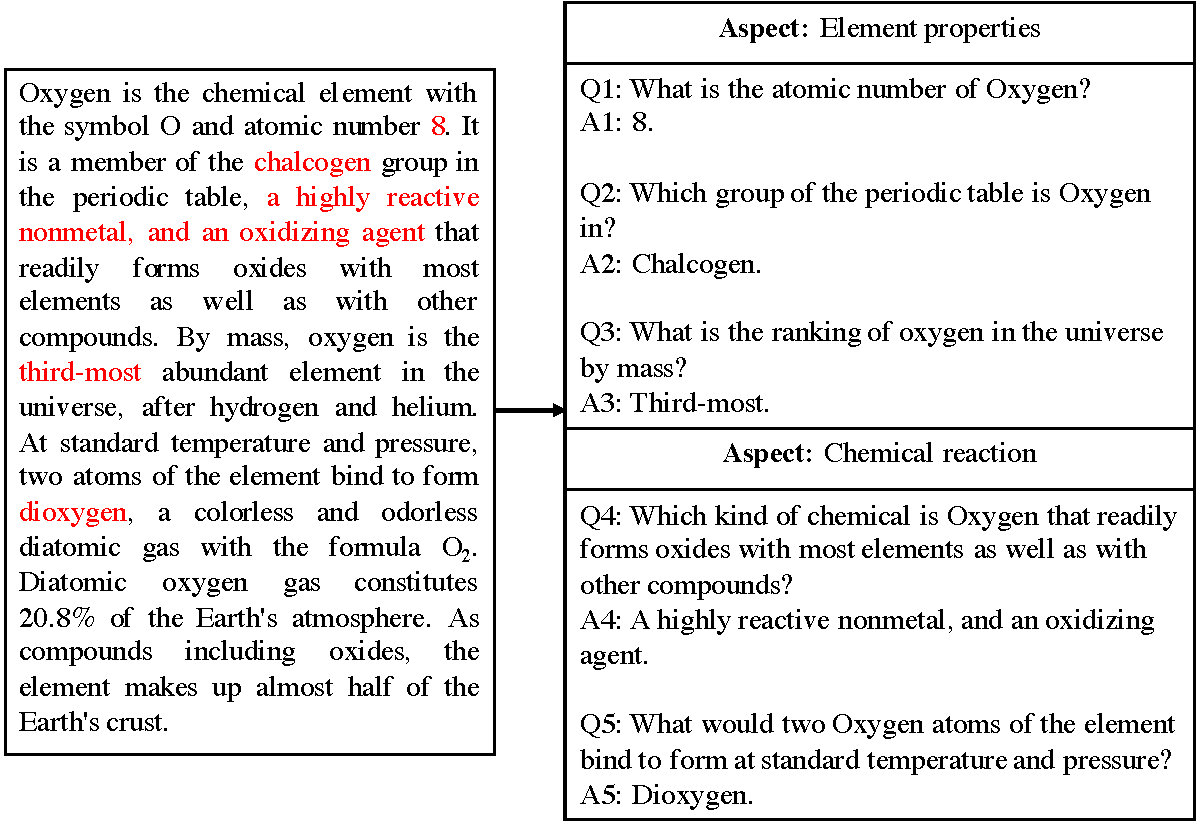
\includegraphics[width=0.5\textwidth]{pic/example.pdf}
	\caption{\label{fig:example} An example of generating different QAs related to different aspects from a document. }
\end{figure}


%Therefore, we design a new scenario where the QA pairs extracted from the documents exist with their corresponding aspects.
In this paper, we propose a variant of the QA generation problem as
illustrated in \figref{fig:process}:
Given a document and an aspect keyword which specify a viewpoint, 
generate a set of QA pairs corresponding to that aspect.

\begin{figure}[th]
	\centering
	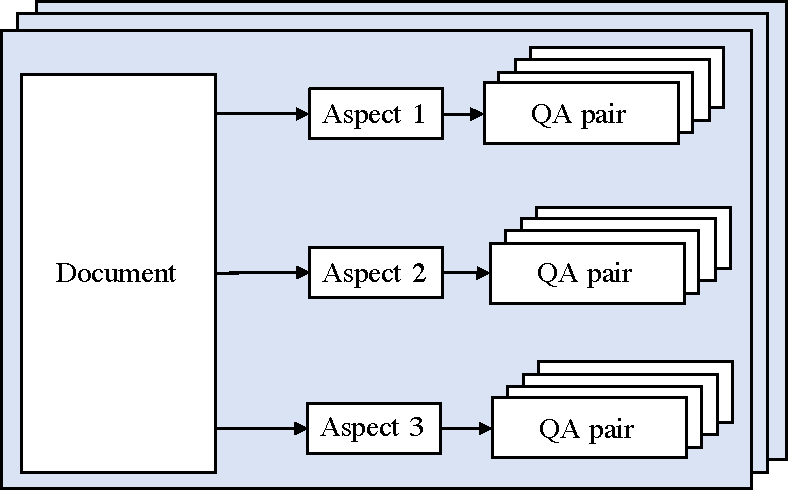
\includegraphics[width=0.35\textwidth]{pic/process.pdf}
	\caption{\label{fig:process} The definition of the aspect-based 
question-answer pairs generation. 
Given a document, the question-answer pairs will be generated 
with the corresponding aspect keywords. 
%\KZ{Better use hint1, hint2 to mean
%that we generate different set of QAs given different hints.}
} 
\end{figure}

Because no dataset exists for this new problem, we construct 
a new type of QA dataset for such scenario with the help of 
SQuAD 2.0~\cite{rajpurkar2018know}. 
SQuAD is a high-quality reading comprehension dataset which contains more than 100,000 questions annotated by human beings. 
It chose 477 documents from Wikipedia and annotated series of QA pairs from 20329 paragraphs.
We crawled the closest heading of each paragraph from the corresponding Wikipedia page as the aspect keyword to this paragraph, and construct the aspect-based QA dataset. For a more accurate testing result, we also manually annotate 11 documents and establish a test set with more than 1000 test cases.
%Figure \ref{fig:wiki} shows an example of Wikipedia page with the information followed by the aspect-based QA dataset.

%\begin{figure}[th]
%	\begin{center}
%	\includegraphics[width=0.48\textwidth]{pic/Wikipedia.eps}
%		\caption{\label{fig:wiki} An example of Wikipedia page \textbf{Mali} and the information followed by our aspect-based QA dataset.
%		The blocked contexts are the paragraph included in SQuAD2.0. The aspect keyword is the closest heading of the paragraph. The QA pairs in the right side is annotated in SQuAD2.0. \KZ{I think this fig should be shown
%in later section where we introduce dataset construction. It helps to
%explain how to create the dataset.}}
%	\end{center}
%\end{figure}

%\KZ{\figref{fig:wiki} needs to show why aspect keyword is important. Need to
%distinguish between the QA pairs from SQUAD and the QA pairs in our
%dataset. I think we can highlight those ones in our datasets, so they
%know the difference between ours and SQUAD.}
%The previous methods to obtain answers can be divided into extractive methods and generative methods. 
%The extractive methods usually use ranking model to select answer phrases from the candidates obtained by lexical features~\cite{witten2005kea,liu2011automatic,wang2016ptr,subramanian2017neural}.
%Sequence labeling and the pointer network are also chosen to extract answers from the source document~\cite{subramanian2017neural}.
%The generative methods can both generate answers from vocabulary and the source text~\cite{meng2017deep,chen2018keyphrase,ye2018semi}.
%The answers can also be generated by reading comprehension methods with the given document and questions.

To solve the problem, we design two frameworks to generate the QA pairs. 
One is a three-step pipeline method which includes paragraph retrieval, answer extraction and question generation. 
Because of the lengthy document, the retrieval step here is designed to search the paragraphs relevant to the aspect keyword.
Another is a filtering method which tries to remain the relevant QA pairs after generation.
%\KZ{What's the wrong with the above two methods? This inspires the
%third approach.} 

%However, multi-step approaches cause terrible error propagation, an end-to-end model is expected to reduce large errors.
%Inspired by the seq-to-seq architecture of UNILM~\cite{dong2019unified},  we design a joint model to generate QA pairs with the document and relevant aspect keywords.
%The main idea of this model is divided into two part: 1) use paragraphs and aspect keywords to extract answer spans from the source document; 2) use paragraphs, aspect keywords and answers to generate questions. 
%The paragraphs and aspect keywords in both parts can share the same UNILM encoder. 

In order to evaluate the entirety of a QA pair, we design an end-to-end metric to calculate the overall score of the generated QA pairs. 

In summary, the contribution of this paper is:
\begin{enumerate}
\item We define a new task that focuses on the aspect-based QA pairs automatic generation.  Because of the requirements of the task, a  QA dataset containing aspect keywords is also constructed.
\item In order to evaluate the quality of the methods, we design an end-to-end metric to calculate the overall score of the generated QA pairs (Section \ref{sec:eval}). To the best of our knowledge, we are the first to evaluate the entirety of a QA pair.
\item We show that adding aspect in the generation model can really play a guiding role in generating QA pairs with a higher degree of relevance to aspect, rather than just using aspect for filtering before or after generation.
%\item We propose a joint architecture AspectQAG to generate QA pairs which outperforms the three-step baseline methods and the filtering strategy substantially by our new defined evaluation metric (Section{\ref{sec:method},\ref{sec:eval}}).
\end{enumerate}

The rest of the paper is organized as follows. In Section \ref{sec:method}, we describe the two frameworks to generate QA pairs. 
In section \ref{sec:data}, we introduce the construction of the aspect-based QA dataset.
Section \ref{sec:eval} talks about the experimental setup and evaluation. 
In Section \ref{sec:related}, we discuss the related work and Section \ref{sec:conclusion} comes the conclusion.
 
